\begin{frame}{Reconhecimento de Voz}{Definição e componentes}

\begin{block}{Definição}
\textbf{Reconhecimento automático de voz} é um campo que desenvolve técnicas para computadores captarem, reconhecerem e traduzirem a linguagem falada para texto; por isso também o nome \textit{speech to text} (STT)
\end{block}

\uncover<2->{
\begin{itemize}
\item Um sistema genérico STT possui três componentes:
\end{itemize}

\begin{figure}
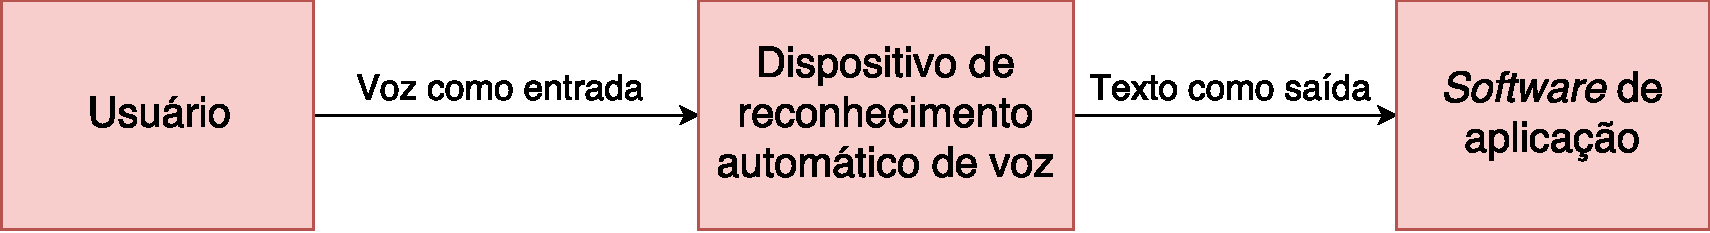
\includegraphics[width=\textwidth]{image/generic-stt.pdf}
\begin{center}
\color{blue}\tiny\cite{sttComponentsParameters}
\end{center}
\end{figure}
}

\end{frame}

% ---------------------------------------------------------------------

\begin{frame}{Reconhecimento de Voz}{Principais termos}

\begin{itemize}
\item \textbf{Fluência}: Forma de comunicação com o sistema
\begin{itemize}
  \item Palavras isoladas
  \item Palavras conectadas
  \item Fala contínua
\end{itemize}

\item<2-> \textbf{Dependência do usuário}: Há treinamento?
\begin{itemize}
  \item Sistemas dependentes
  \item Sistemas independentes
\end{itemize}

\item<3-> \textbf{Vocabulário}: Palavras reconhecidas pelo sistema

\item<4-> \textbf{\textit{Utterance}}: Vocalização de palavras
\end{itemize}
\end{frame}
